\documentclass{article}

\title{Distributed sorting using Apache Arrow Flight for communication}
\author{Chengxin Ma}
\date{\today}

\usepackage{graphicx}
\usepackage{hyperref}
\usepackage{todonotes}

\begin{document}

\maketitle

\section{Introduction}
This report includes the design and implementation of a distributed sorting application which utilizes Apache Arrow Flight for communication.

\section{Design}
\subsection{Test data}
The final goal of designing this application is to integrate it into a genomic data process pipeline, where data in the SAM format
\footnote{\url{https://en.wikipedia.org/wiki/SAM_(file_format)\#Format}} is sorted.

From the perspective of sorting, the most interesting fields are \texttt{RNAME} (the name of the references sequence) and \texttt{POS} (position).
They together determine the order in which records are sorted.

Thus, to simplify the prototyping work, we design a data structure with three fields: \texttt{GROUP}, \texttt{SEQ}, and \texttt{DATA}.
Each record belongs to a group and has a sequence number in that group.
Its data is placed in the \texttt{DATA} field.

Here is an example input file: \href{https://github.com/MaChengxin/playground/blob/master/arrow/flight/my_flight/data/4_nodes/records_on_node_0.txt}{\textit{Input records on Node 0}},
and here is an example file containing expected sorted records: \href{https://github.com/MaChengxin/playground/blob/master/arrow/flight/my_flight/data/4_nodes/expected_records_on_node_0.txt}{\textit{Expected sorted records on Node 0}}.
Note that we do not necessarily need to write the output into files.
It is only for experimenting purpose.
After integration we could use in-memory storage instead.

\subsection{Functional decomposition}

The following functional components must be implemented to complete the application.
\begin{itemize}
    \item sorter
    \item sender and receiver
    \item partitioner and merger
    \item storage
\end{itemize}

The \textit{sorter} is responsible for sorting the data in our desired order: records with smaller Group IDs are placed before those with large Group IDs.
If the Group IDs of two records are the same, the secondary criteria is the sequence number.

The \textit{sender} and \textit{receiver} are responsible for sending data to destination nodes and receiving data from source node respectively.

The responsibility of the \textit{partitioner} is to partition the data into different groups that would be sent to different destinations,
while the \textit{merger} is to merge the partitioned data to a complete set.

\textit{Storage} is needed when we want to temporarily store the data before further processing.

\section{Implementation}
There are some dependencies among the functional components.
The \textit{sender} must wait until \textit{partitioner} has partitioned the inputs to groups with known destination.
The \textit{merger} must wait until the \textit{receiver} has got all the data, and then the \textit{sorter} can perform its task.

Thus, the current implementation runs three processes on each node:
\textit{partition-and-send},
\textit{receive-and-sort}, and
\textit{plasma-store-server}.

The following tables show the steps in \textit{partition-and-send} and \textit{receive-and-sort}.
For \textit{plasma-store-server}, the only step is to start it.

\begin{table}[h!]
    \centering
    \begin{tabular}{|l|l|}
    \hline
           & \multicolumn{1}{c|}{\textbf{Partition and Send}} \\ \hline
    Step 1 & Read data from input file into memory.           \\ \hline
    Step 2 & Partition the in-memory data.                    \\ \hline
    Step 3 & Put partitioned data to Plasma.                  \\ \hline
    Step 4 & Retrieve from Plasma and send to other nodes.    \\ \hline
    \end{tabular}
    \caption{Steps in the partition-and-send processes}
\end{table}

\begin{table}[h!]
    \centering
    \begin{tabular}{|l|l|}
    \hline
           & \multicolumn{1}{c|}{\textbf{Receive and Sort}}                     \\ \hline
    Step 1 & Start the Flight server, waiting for data from other nodes.        \\ \hline
    Step 2 & Receive data from other nodes, put into Plasma, increment counter. \\ \hline
    Step 3 & When all data received, retrieve data from Plasma.                 \\ \hline
    Step 4 & Sort the retrieved data.                                           \\ \hline
    Step 5 & Write sorted data to output file for verification.                 \\ \hline
    \end{tabular}
    \caption{Steps in the receive-and-sort processes}
\end{table}

\subsection{Test run}
To see the performance of the application, a test run has been performed.
4 nodes on Cartesius (\texttt{tcn348, tcn918, tcn1354, tcn1540}, we name them from Node 0 to 3 hereafter) were allocated for this test run.
The data for the test run contains records of 40 groups (from \texttt{GROUP0} to \texttt{GROUP39}), each having 1 million records (i.e. the total number of records is 40 million).
Each node had 10 million records in random order before the application ran, and we expected that after when the application finishes,
Node 0 stores records from \texttt{GROUP0} to \texttt{GROUP9},
Node 1 stores records from \texttt{GROUP10} to \texttt{GROUP19},
Node 2 stores records from \texttt{GROUP20} to \texttt{GROUP29},and
Node 3 stores records from \texttt{GROUP30} to \texttt{GROUP39}, in the ascending order.

The size of the input and output files on each node is around 270 MB.

The test run was started one by one manually, in the order of from Node 0 to 3.
The following picture shows the key moments on these four nodes.
\footnote{Data source: \url{https://docs.google.com/spreadsheets/d/1xP0lDKG_e8G8zPHNXfgWH1iLae2SFBsvTdGjZgrteWA/edit?usp=sharing}}

\begin{figure}[h!]
    \caption{Key moments in distributed sorting test run with 4 nodes}
    \centering
      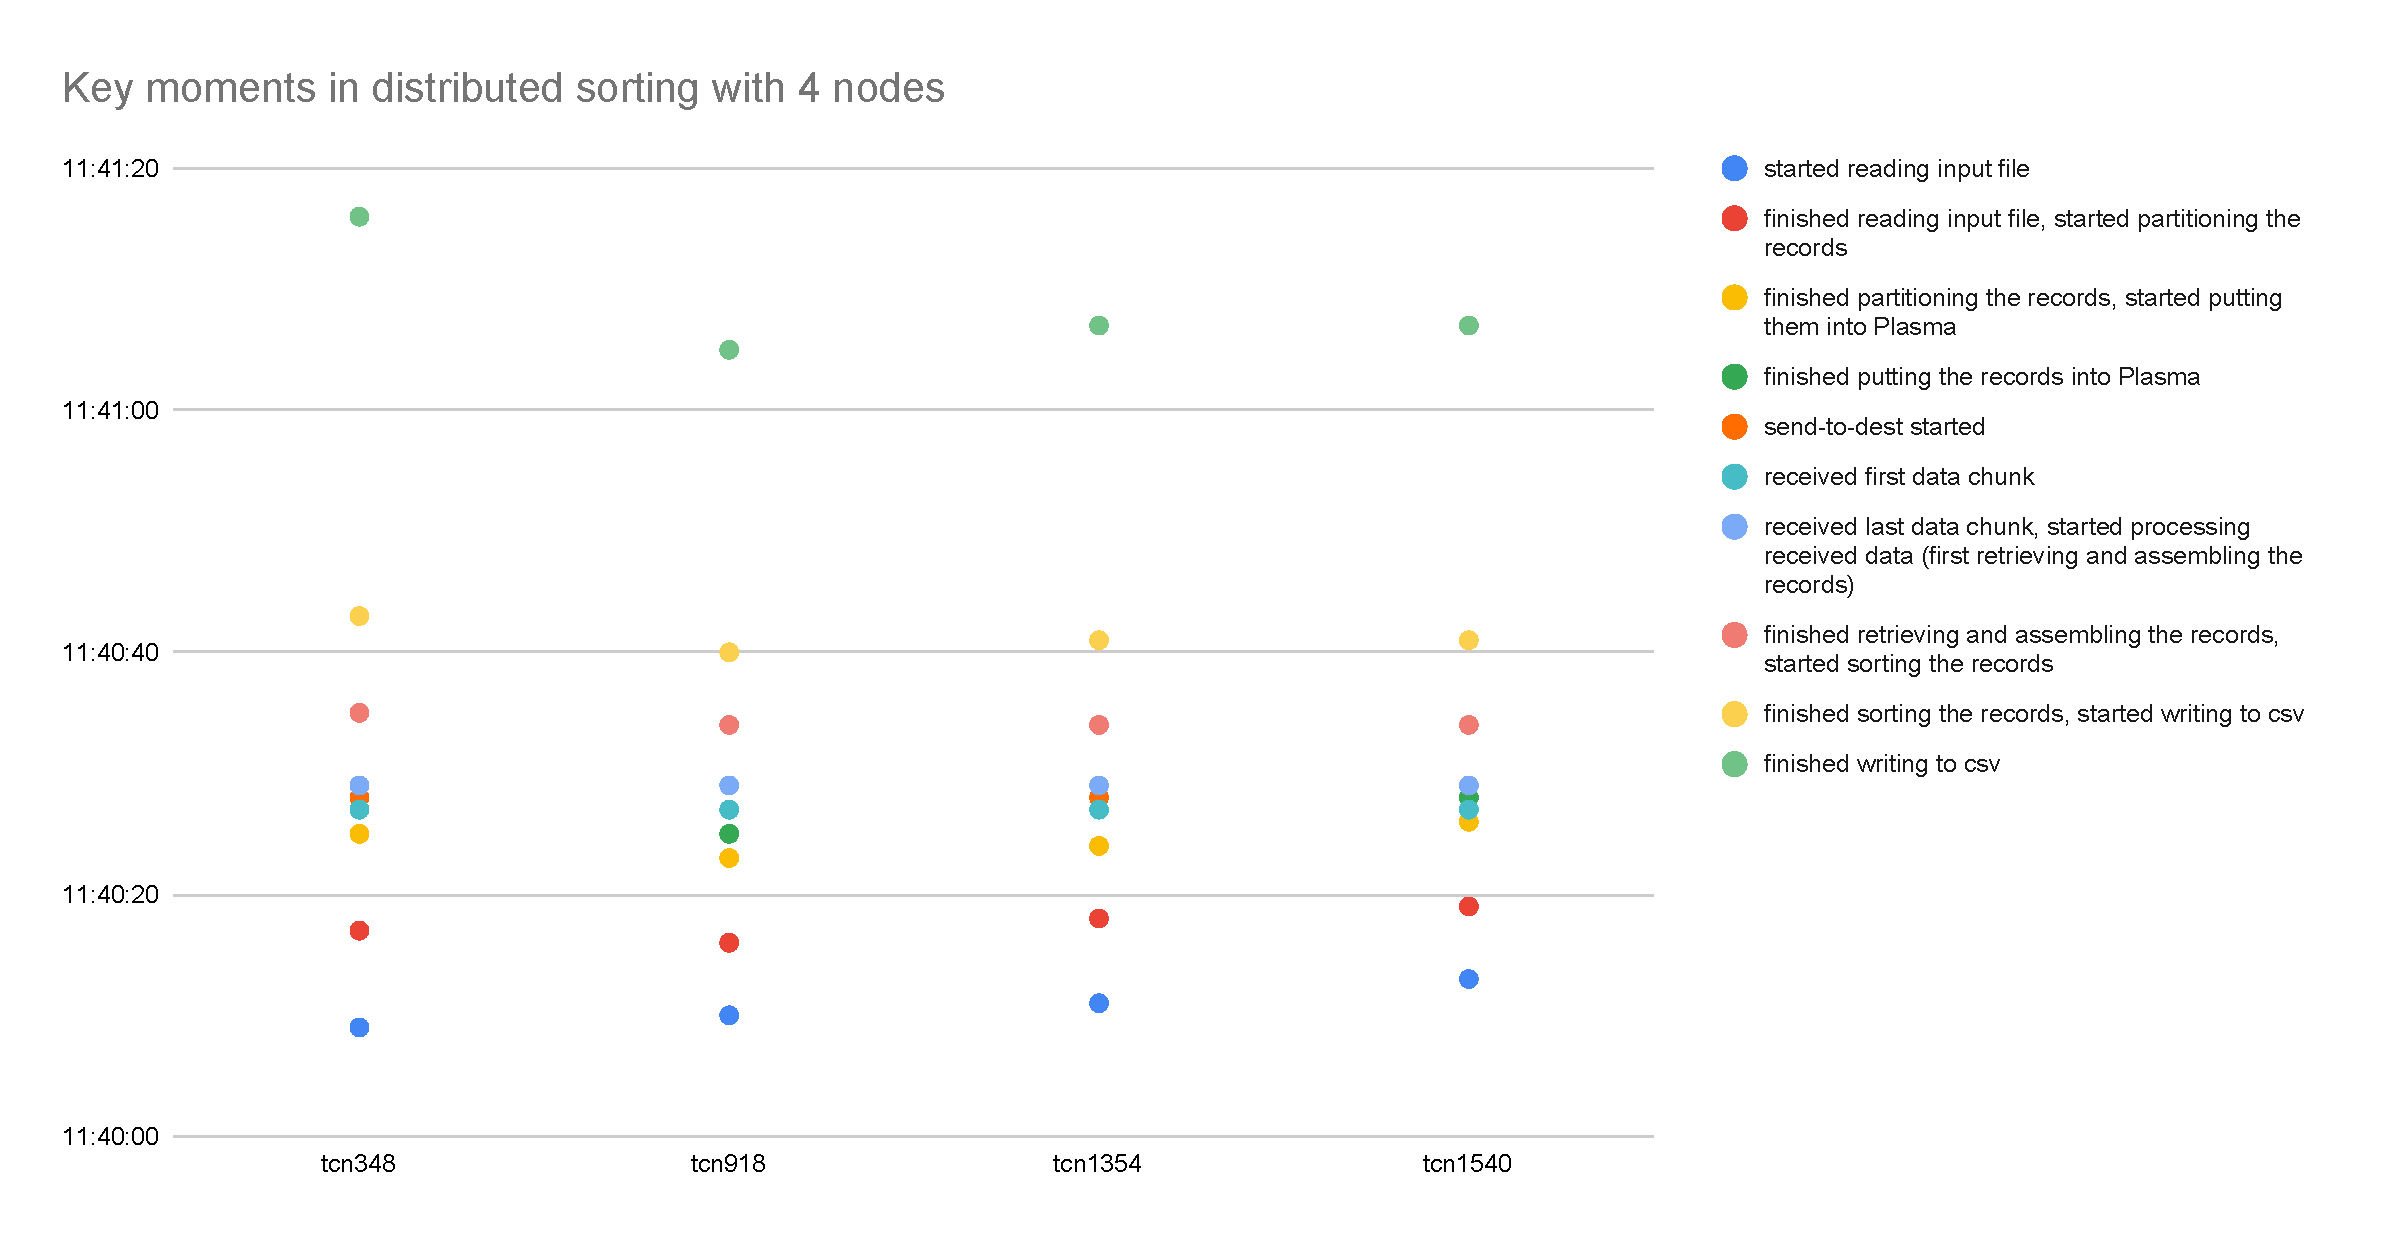
\includegraphics[width=1.4\textwidth]{key_moments}
  \end{figure}

We can see that the performance on the four nodes is more or less the same, except that on \texttt{tcn348} it took a bit longer to write to the output files.

In this test run, the first task was to read the data from the input file.
It took around 7 seconds.
Note that there is no such step after the distributed sorting application has been integrated to the whole genomic pipeline,
as its previous step could store the temporary results in memory.

After the input data had been loaded into memory as \texttt{pandas DataFrame}, the next task is to partition it according to some criteria.
In this case, since we have four nodes, the data was partitioned to 4 subsets, and later they were stored to \texttt{Plasma Object Store}.
Partition took about 8 seconds while putting the partitioned data to the in-memory store took about 2 seconds.

At this moment, the \textit{sender} was ready to send away to the data to the destination nodes.

The receiving process on every node would put received data to \texttt{Plasma} and increment a counter counting how many datasets had arrived.
If the \textit{receiver} had observed that it had got all the data, the data processing part (merge and sort) would begin.

On each node, starting sending data to other nodes marks the beginning of the communication phase, while receiving the last piece of data marks the end of the communication phase.
Note that the receiving part is dependent on other nodes.

In this test run, the communication phase on each node took roughly 2 seconds.
The overall communication phase (marked by earliest sending and latest receiving on \textbf{all} nodes) is also about 2 seconds since each node's communication phase overlapped with other nodes'.

To process the received data, first it was needed to be retrieved from \texttt{Plasma}.
It took about 5 seconds.

After that it was the sorting task, which took approximately 6 seconds.

Finally, the sorted records were written to \texttt{csv} files for verification.
It took about 26 seconds on 3 nodes, and on the other node it took 33 seconds.
Like reading from input data, these step in not needed after integration.

Ignoring the abnormal writing to disk time on \texttt{tcn348}, we can see that the overall execution time is about 56 seconds, in which:
\begin{itemize}
    \item file I/O (reading from and writing to \texttt{csv} files) took 32 seconds;
    \item in-memory store access took 7 seconds;
    \item communication (sending and receiving records) took 3 seconds;
    \item partitioning took 8 seconds;
    \item sorting took 6 seconds.
\end{itemize}

Since disk I/O can be removed after integration, we remove this task and plot the remaining ones in Figure \ref{fig:time_of_tasks}.

\begin{figure}[h!]
    \caption{Time spent on different tasks (disk I/O removed)}
    \centering
      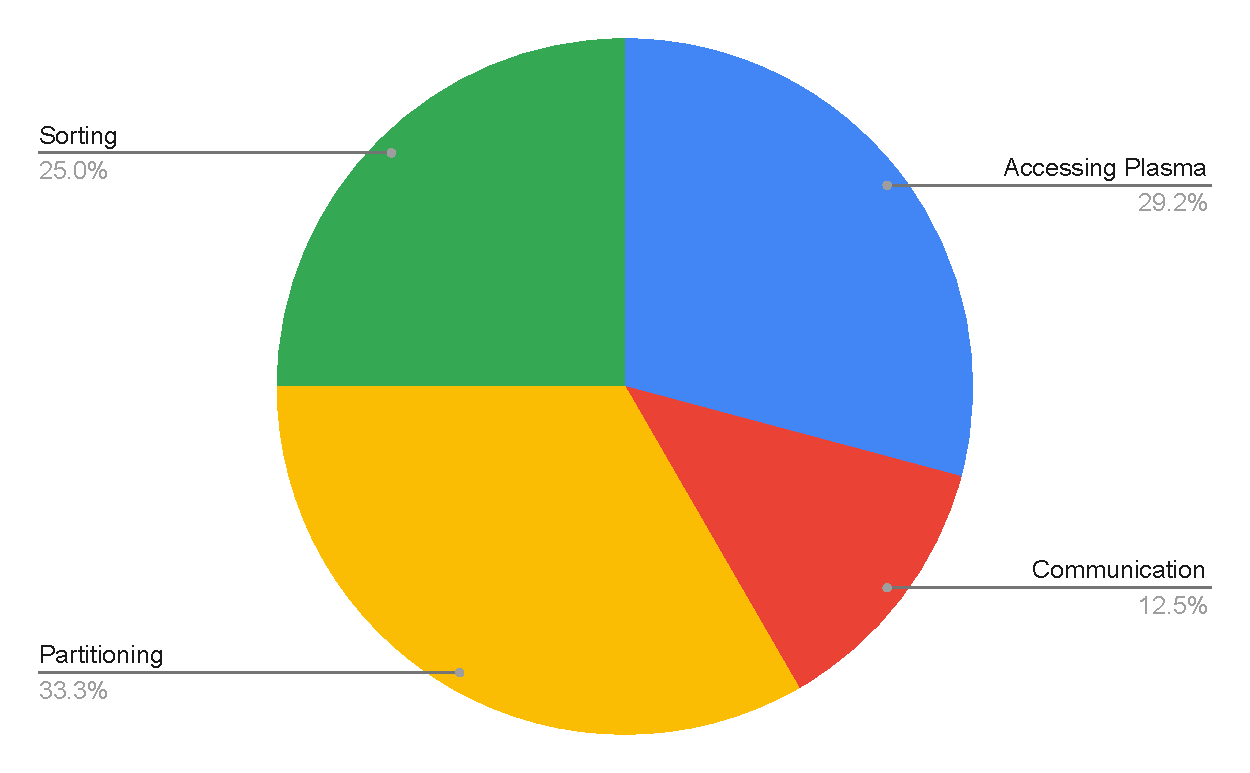
\includegraphics[width=0.8\textwidth]{time_of_tasks}
    \label{fig:time_of_tasks}
\end{figure}

We see that only a quarter of the time is spent on sorting.
The other tasks are required to perform \textbf{distributed} sorting.
It will be interesting to ask: 

\textit{Is it worth the effort to distribute the sorting task to multiple nodes?}
\footnote{In the test run, we can predict that if we use only one node to sort all the data,
the time of partitioning, accessing Plasma, and communication will be all gone,
 but the sorting time will be a bit more than 4 times than the current sorting time (assuming $O(n\log{}n)$ complexity).
So the overall time might be a bit more than distributed sorting.}

\section{Experiments}
\todo[]{TODO}

The goal of the experiments is to determine:
\begin{itemize}
    \item Does the performance become better if more nodes are used?
    \item How does the application behave when the volume of data increase?
    \item Where is the bottleneck of performance?
\end{itemize}

\subsection{Input size fixed, changing the number of nodes in use}

\subsection{Number of nodes fixed, changing the input size}

\newpage
\appendix
\section{Known issues}
\subsection{Building the project}

On macOS, the \texttt{grpc} library installed via \texttt{Homebrew} (as a dependency of \texttt{apache-arrow}) seems to be problematic.
The Flight server would incur a segmentation fault due to the current version (stable 1.26.0) of \texttt{grpc}.

We can make use of the existing build system of arrow to build \texttt{grpc} from source.
(The build system is capable of building any missing dependency from source.)
This also saves us from building missing dependencies manually on Cartesius.

\end{document}
